\RequirePackage{fix-cm}
\documentclass[compress]{beamer}
\RequirePackage{fahrenberg}
\newcommand*\flow{\textup{\textsf{flow}}}
\newcommand*\exit{\textup{\textsf{exit}}}
\newcommand*\inv{\textup{\textsf{inv}}}
\newcommand*\mlbrace{\mathopen{\{\!\!\{}}
\newcommand*\mrbrace{\mathclose{\}\!\!\}}}

\begin{document}

\begin{frame}[plain]
  \centering
  \includegraphics[width=\textwidth]{dhs1}
\end{frame}

\begin{frame}[plain]
  \centering
  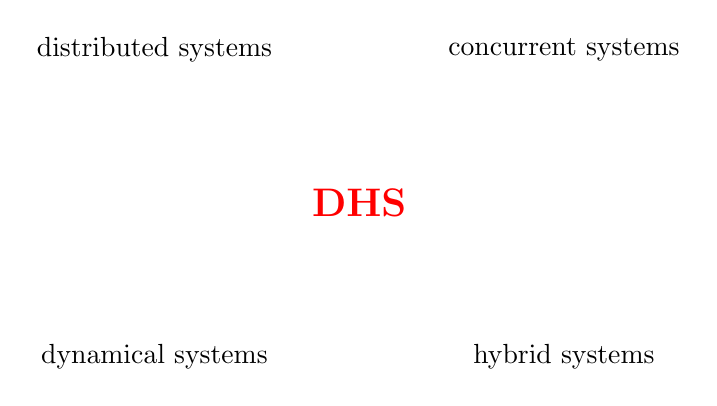
\begin{tikzpicture}[scale=1.3]
    \node at (0,0) {distributed systems};
    \node at (4,0) {concurrent systems};
    \node at (0,-3) {dynamical systems};
    \node at (4,-3) {hybrid systems};
    \node at (2,-1.5) {\Large \color{red} \bf DHS};
  \end{tikzpicture}
\end{frame}

\begin{frame}[plain]
  \centering\bigskip
  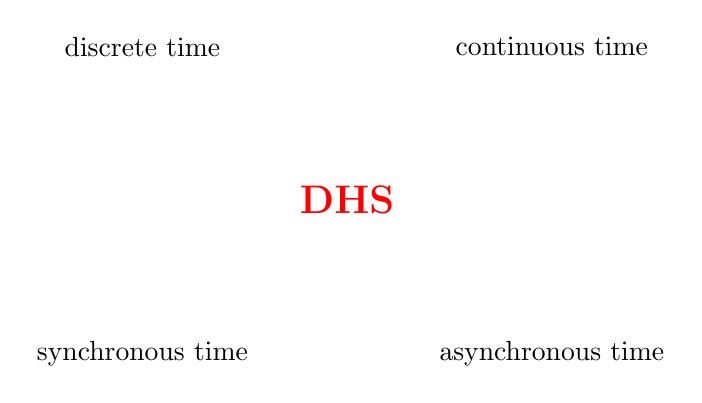
\begin{tikzpicture}[scale=1.3]
    \node at (0,0) {discrete time};
    \node at (4,0) {continuous time};
    \node at (0,-3) {synchronous time};
    \node at (4,-3) {asynchronous time};
    \node at (2,-1.5) {\Large \color{red} \bf DHS};
  \end{tikzpicture}
\end{frame}

\begin{frame}[plain]
  \centering
  \includegraphics[width=\textwidth]{dhs2}

  \bigskip Alessandro Abate \qquad Martin Fr{\"a}nzle \qquad Kim G. Larsen
  \\
  Martin Raussen \qquad Rafael Wisniewski
\end{frame}

\begin{frame}[plain]
  \centering
  \includegraphics[width=\textwidth]{dhs3}
\end{frame}

\begin{frame}[plain]
  \centering
  \includegraphics[width=\textwidth]{dhs4}
\end{frame}

\begin{frame}[plain]
  \textbf{Informal workshop dinner}: \\
  \textbf{19:30}, Cr{\^e}perie La Belle Ronde, 19 rue Daguerre, Paris 14

  \centering\medskip
  \includegraphics[width=\textwidth]{dhs5}
\end{frame}



\end{document}

